\section{Theory}
\label{sec:theory}
The aim of this experiment is to record the absoption spectrum
of rubidium. Therefore a diode laser is adjusted and aimed towards a cell
filled with rubidum.
The following sections introduce the theory
important for the understanding of the experiment.

\subsection{Laser basics}
\label{subsec:Laser}
A Laser (Light Amplification by Stimulated Emission of radiation)
emits highly intensive light with a long coherece length.
Fist of all the interaction of a radiation field with
a energy level system is considered. These includes
absoption and spontaneous and stimulated emission
of a photon, shown in figure \ref{fig:ab_em}.
\begin{figure}
\centering
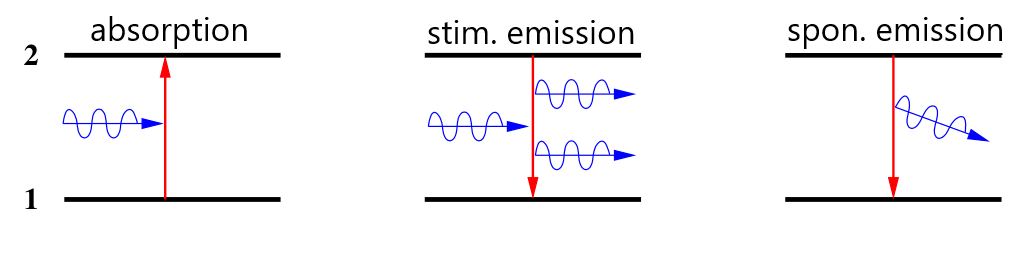
\includegraphics[width=0.7\textwidth]{ab_und_emiss.png}
\caption{Absorption and both spontaneous and stimulated emission of a photon in a two energy level system.
\cite{V61}}
\label{fig:ab_em}
\end{figure}
Absorption descripts the process where a photon annihilates and
delivers energy for the transition
to a higher energy level.
Spontaneous emission discripts the opposite, a photon is
emitted if a transition to a lower energy
level occurs spontaneously.
But most important for a laser as the name indicates
is the stimulated emission.
The process of stimulated emission works as follows.
If a photon with the energie same as
the energy gap between the two energy levels
encounters an excited state, an other photon with
same energy and phase is emmitted and the excited state
returns to the ground state.
To run a laser stimulated emission must be the commonest interaction.
But the occupation of the energy levels for fermion follows
the Fermi-Dirac statistics so higher levels are
less occupied. By increases the temperature only
a same occupation can be accomplish.
However, this is not enough in order to ensure mostly stimulated emission.
Therefore a
population inversion between ground state and an excited
state is necessary.
As to achieve this at least a three level system is of need.
Transitions between the levels can be radiative as explained above
aswell as non radative for example in the form of lattice vibration.
But the decay rate of the level

non radative
radative


To accomplish laser radiation, some criteria must be met.
First of all a gain medium is necessary in which
a population inversion by pumping is created.
Pumping energy is supplied by light or electric current.
The Laser cavity consists of the gain medium and two
mirrors, one higly reflective and the other
partially transparent,
the output coupler.
In the figure \ref{fig:laserschema}
a schematic laser with its components is displayed.
\begin{figure}
\centering
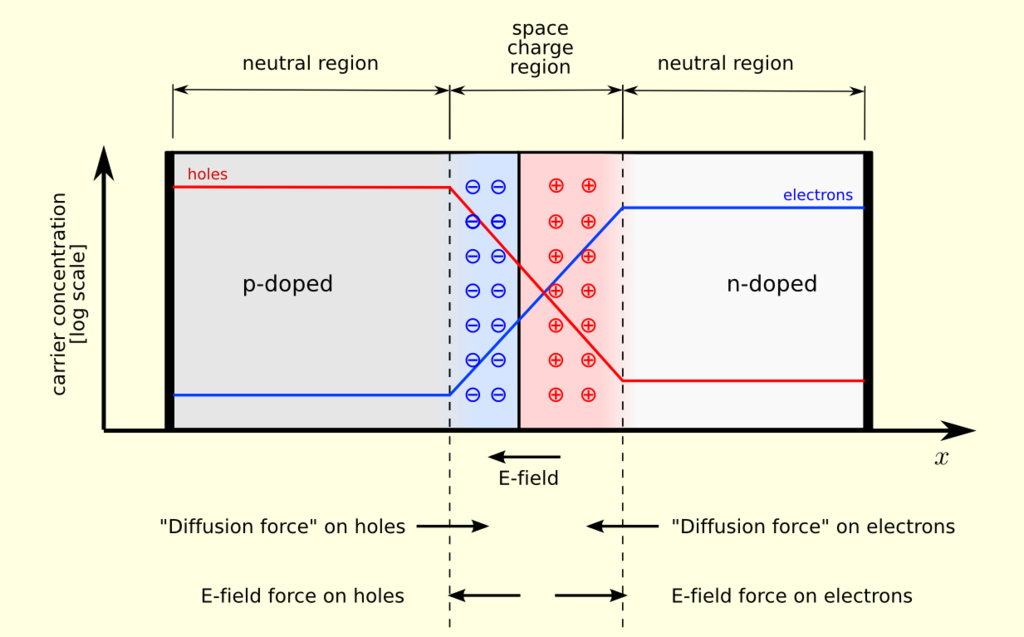
\includegraphics[width=0.7\textwidth]{equilibrium.png}
\caption{A schematic Laser and its components.
\cite{wiki_diode}}
\label{fig:equi}
\end{figure}

The operation of the Laser cavity is as followed.
Photons are emitted through spontaneous emission
in the gain medium. The two mirrows
ensure that the photons stay in the Laser cavity
and the Laser intenensity increases due to
stimulated emission of other photons.


\subsection{Semiconductor}
\label{subsec:Semiconductor}

The diode laser is a result of the reseaching done on semiconductor.
So first a deeper comprehension of semiconductor theory is needed.
Hence the principle funcion of a simple p-n diode is described.
A p-n diode exist out of two semiconductor materials one
n-type and the other p-type.
In the p-type semiconductor is an excess of holes
and in the n-type semiconductor, an exess of electrons.
An excess of holes or electrons can be accomplish by doping.
When n- and p-type are merged together,
electrons and holes diffuse in opposite side and recombine.
This process induce a elctricfield bettween the fixed doping atoms, which
counteracts the diffusion process.
If equilibrium between the two forces is accomplish
a charge depletion zone is created
at the p-n junction.
The figure \ref{fig:equi} shows
a schematic p-n Diode in equilibrium.

\begin{figure}
\centering
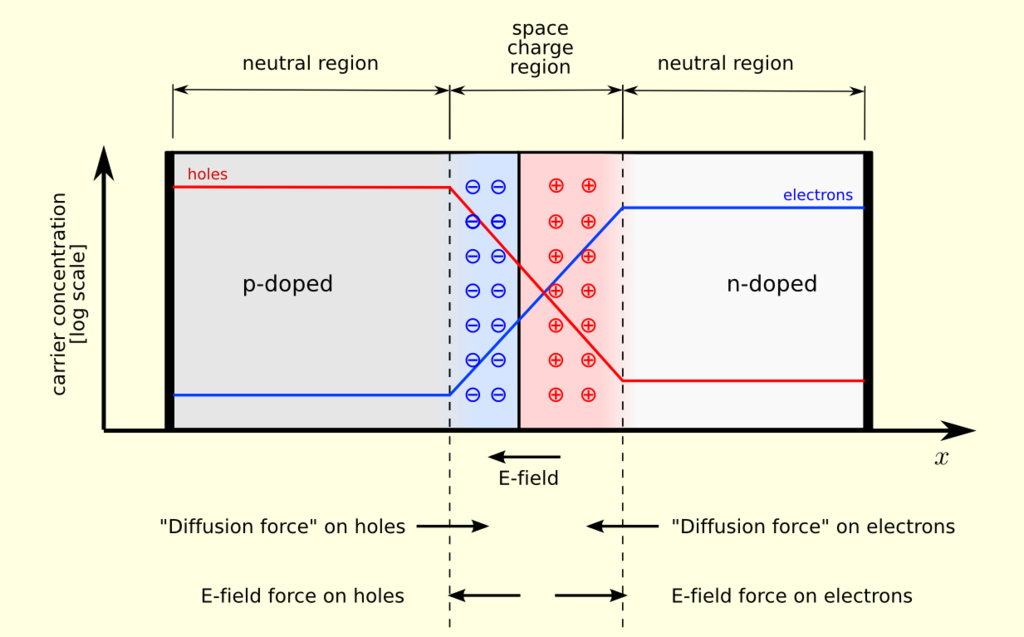
\includegraphics[width=0.7\textwidth]{equilibrium.png}
\caption{A schematic p-n Diode in equilibrium.
\cite{wiki_diode}}
\label{fig:equi}
\end{figure}

There are two possible ways apply voltage
in forward bias and
in rewerse bias.
In forward bias the diode let the curruent follow
but in the rewese bias the diode bocks the current up to the breaking point.
A typical diode characteristic is shown in figure \ref{chara}
\begin{figure}
\centering
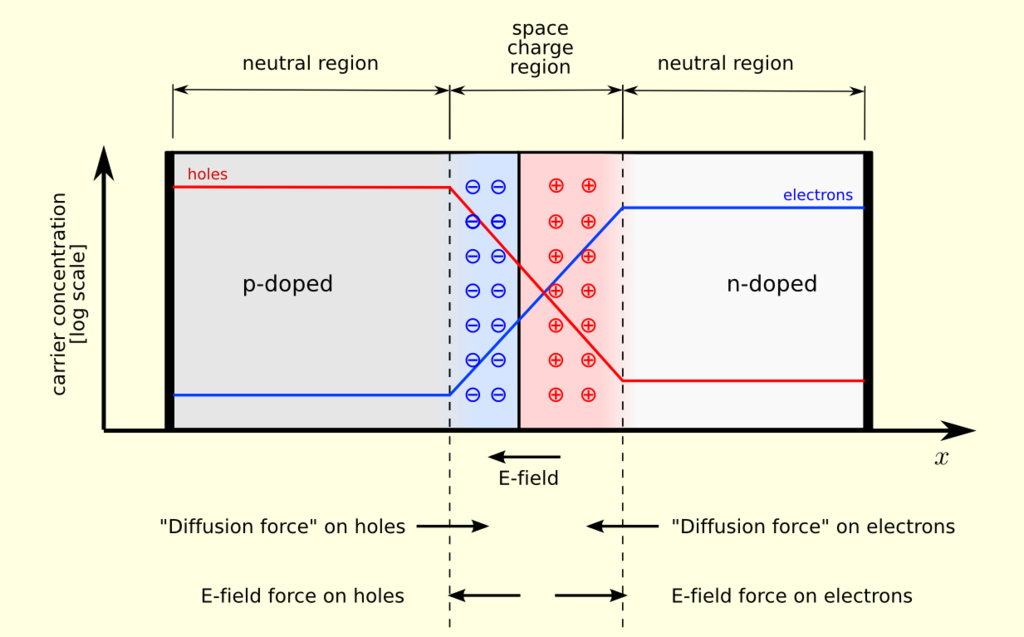
\includegraphics[width=0.7\textwidth]{equilibrium.png}
\caption{A schematic p-n Diode in equilibrium.
\cite{sparkfun}} % https://learn.sparkfun.com/tutorials/diodes/real-diode-characteristics
\label{fig:chara}
\end{figure}
For the Diode Laser a light-emitting diode (LED)
is necessary. A LED differ in terms of
the band gab
from a simple p-n diode.
For a LED a direct band gab is needed, so a photon
with the energy of the band gab is
emitted if electrons and holes recombine.


\begin{figure}
  \centering
  \includegraphics{plot.pdf}
  \caption{Plot.}
  \label{fig:plot}
\end{figure}



\subsection{Diodenlaser}
\label{subsec:diodenlaser}


\subsection{Beiträge im Laser}
\label{subsec:}



\subsection{Rubidum spektrum}
\label{subsec:}


\subsection{piezo}
\label{subsec:}
